% Informe de laboratorio 6: analisis de datos de entrada y bondad de ajuste
% Formato IEEE, doble columna (IEEEtran conference).
% Compilar con pdflatex (dos pasadas) desde esta carpeta. Las figuras se leen de ../figuras
% y las tablas numericas de tablas/, generadas por tablas_latex.py a partir de los CSV.
\documentclass[conference]{IEEEtran}

\usepackage[T1]{fontenc}
\usepackage[utf8]{inputenc}
\usepackage[spanish,es-nodecimaldot,es-tabla]{babel}
\usepackage{graphicx}
\usepackage{amsmath,amssymb}
\usepackage{booktabs}
\usepackage{array}
\usepackage{url}
\usepackage{cite}
\usepackage{balance}

\graphicspath{{../figuras/}}

% \input no es expandible justo antes de \bottomrule; se usa la primitiva de TeX
\makeatletter\newcommand{\tabla}[1]{\@@input tablas/#1.tex }\makeatother

\hyphenation{log-nor-mal log-lo-gís-ti-ca Wei-bull}

\begin{document}

\title{Análisis de datos de entrada y bondad de ajuste de distribuciones de probabilidad}

\author{\IEEEauthorblockN{Santiago Barrera Meza}
\IEEEauthorblockA{Código 160005004\\
Simulación Computacional, Universidad de los Llanos\\
sbarrera.meza@unillanos.edu.co}}

\maketitle

\begin{abstract}
Este informe desarrolla la práctica de análisis de datos de entrada (formato FO-DOC-112). Se analizan cuatro muestras de 200 tiempos entre llegadas (A, B, C y D): primero con estadística descriptiva, después con las gráficas heurísticas de independencia y estabilidad de Banks, y por último ajustando nueve distribuciones por máxima verosimilitud, comparadas con SSE, AIC y BIC. B y D se comportan como muestras IID. B se describe bien con una Weibull de forma $0.91$, muy cerca de una exponencial de media 0.205, y D con una lognormal de $\sigma=1.02$. A es estacionaria pero correlacionada ($r_1=0.49$), así que la normal que mejor la ajusta solo describe su distribución marginal. C no es estacionaria: la media de su segunda mitad es 2.65 veces la de la primera. La gamma que mejor la ajusta mezcla dos regímenes y no debería usarse como modelo único. Los cuadernos adjuntos contienen el código, los datos y todas las salidas.
\end{abstract}

\begin{IEEEkeywords}
datos de entrada, independencia, estacionariedad, ajuste de distribuciones, AIC, BIC, máxima verosimilitud
\end{IEEEkeywords}

%--------------------------------------------------------------------
\section{Introducción}
Un modelo de simulación es tan bueno como sus entradas. Antes de elegir una distribución para los tiempos entre llegadas o de servicio hay que comprobar si los datos se pueden tratar como una muestra IID; si no se puede, ninguna distribución ajustada a toda la muestra los representará bien~\cite{banks98}.

La guía~\cite{guia} pide tres pasos con cuatro conjuntos de datos: estadística descriptiva (5.1), análisis de independencia y estabilidad (5.2) y ajuste de distribuciones con medidas de bondad de ajuste (5.3). El informe sigue ese orden después de responder la consulta previa. El análisis de 5.1 y 5.2 está en \texttt{Lab6\_160005004\_analisis\_entrada.ipynb} y el de 5.3, en un cuaderno aparte, \texttt{Lab6\_160005004\_ajuste\_curvas.ipynb}, como pide la guía.

%--------------------------------------------------------------------
\section{Consulta previa}
\subsection{Estadística descriptiva}
Es la parte de la estadística que resume una muestra sin hacer inferencias sobre la población: medidas de tendencia central (media, mediana), de dispersión (varianza, desviación estándar, rango, rango intercuartílico), de forma (asimetría, curtosis) y de posición (percentiles), junto con tablas y gráficas como histogramas o diagramas de caja. En simulación es el primer filtro: indica el rango de los datos, si hay valores atípicos y qué familias de distribuciones conviene probar.

\subsection{Asimetría, curtosis y percentiles}
La asimetría (\emph{skewness}) mide qué tan desigual es la distribución alrededor de la media: $g_1=m_3/m_2^{3/2}$, donde $m_j$ es el $j$-ésimo momento central. Vale cero en una distribución simétrica y es positiva cuando la cola derecha es más larga, como en los tiempos de servicio. La curtosis, $m_4/m_2^2$, mide el peso de las colas; se suele reportar el exceso respecto a la normal ($m_4/m_2^2-3$), que es cero para la normal y 6 para la exponencial. El percentil $p$ es el valor por debajo del cual queda el $p$\,\% de los datos; Q1, Q2 (mediana) y Q3 son los percentiles 25, 50 y 75.

\subsection{Supuesto IID}
Un conjunto de variables aleatorias $X_1,\dots,X_n$ es IID cuando las variables son \emph{independientes} (conocer el valor de una no cambia la distribución de las demás) e \emph{idénticamente distribuidas} (todas tienen la misma función de distribución $F$). Es el supuesto que justifica ajustar una sola distribución a la muestra y generar en la simulación valores independientes de ella~\cite{banks98}.

\subsection{Proceso estocástico estacionario}
Un proceso $\{X_k\}$ es estacionario (en sentido estricto) si la distribución conjunta de cualquier grupo de variables no cambia al desplazarlas en el tiempo; en particular, la media y la varianza no dependen de $k$. En sentido débil basta con que la media sea constante y la covarianza entre $X_k$ y $X_{k+h}$ dependa solo de $h$. Un proceso no estacionario es, por ejemplo, la llegada de clientes a un restaurante, cuya tasa cambia durante el día.

\subsection{Proceso estocástico correlacionado}
Es un proceso en el que valores cercanos en la secuencia no son independientes: $\mathrm{Cov}(X_k,X_{k+h})\neq0$ para algún $h\ge1$. Se mide con la autocorrelación de retraso $h$. Un ejemplo es un tiempo entre llegadas que depende del anterior, como el conjunto 6 del cuaderno de clase, donde $X_k=\alpha X_{k-1}+(1-\alpha)U_k$. Aunque cada $X_k$ tenga la misma distribución marginal, muestrear valores independientes de esa marginal no reproduce las rachas del proceso real.

%--------------------------------------------------------------------
\section{Metodología}
\subsection{Datos}
Los cuatro archivos se descargaron de los enlaces de la guía. Cada uno tiene 200 valores positivos, que se tratan como tiempos entre llegadas sucesivas, igual que en el cuaderno de clase \emph{Example. Input Data Analysis}. Con esa lectura, el instante de la llegada $i$ es $t_i=\sum_{j\le i}x_j$ y el horizonte $T$ de cada conjunto es la suma de sus valores: 39.0 en A, 41.1 en B, $1.52\times10^{5}$ en C y 412.1 en D.

\subsection{Independencia y estabilidad}
Se usaron las cinco gráficas de la guía con las funciones del cuaderno de clase, con dos ajustes. En el conteo de llegadas, el original guarda el conteo del intervalo $k$ en la posición $k-1$, lo que corre las barras un lugar; aquí cada conteo queda en su intervalo. En la media móvil se usó una ventana de 40 datos ($W=20$ a cada lado) en lugar de 100, porque con 200 datos una ventana de 100 promedia la mitad de la muestra en cada punto. Siguiendo el material de clase~\cite{clase}, las gráficas son el criterio principal y se reacciona solo ante la evidencia más clara en contra; las cifras de la Tabla~\ref{tab:iid} solo las cuantifican. La banda de referencia para las correlaciones es $\pm2/\sqrt{n}=\pm0.141$.

\subsection{Ajuste de distribuciones}
Se ajustaron por máxima verosimilitud con \texttt{scipy.stats}~\cite{amat2021,scipy} las cinco distribuciones de la guía y cuatro adicionales: Weibull, log-logística, gaussiana inversa y Pareto generalizada. Se eligieron para cubrir colas ligeras, intermedias y pesadas, porque las asimetrías de los conjuntos van de $-0.29$ a $3.18$. Como todos los datos son positivos, las distribuciones con soporte $[0,\infty)$ se ajustaron con localización fija en cero. La beta necesita un soporte acotado; se tomó $[\min x - \delta,\ \max x + \delta]$ con $\delta=(\max x-\min x)/(n-1)$ y se estimaron sus dos parámetros de forma. Como los extremos salen de los datos, para la beta se cuentan $k=4$ parámetros.

Con $\ln L$ el logaritmo de la verosimilitud en los parámetros estimados y $k$ el número de parámetros libres:
\begin{align}
\mathrm{AIC} &= 2k - 2\ln L, \qquad \mathrm{BIC} = k\ln n - 2\ln L, \\
\mathrm{SSE} &= \textstyle\sum_{j=1}^{20}\big(h_j - f(c_j;\hat\theta)\big)^2,
\end{align}
donde $h_j$ es la densidad del histograma de 20 particiones y $c_j$ el centro de la partición $j$. En AIC y BIC, menor es mejor; BIC castiga más los parámetros adicionales. El SSE depende de la escala de los datos (por eso en C es del orden de $10^{-8}$) y solo sirve para comparar distribuciones dentro de un mismo conjunto. Como el material de clase recomienda no depender de una sola medida, también se reporta el estadístico de Kolmogórov-Smirnov $D$ (sin su valor $p$, que no es válido cuando los parámetros se estiman con los mismos datos) y se revisan gráficas Q-Q. Las tres mejores se ordenan por AIC; una diferencia de AIC menor que 2 se considera un empate práctico.

%--------------------------------------------------------------------
\section{Estadística descriptiva (punto 5.1)}
\begin{table}[t]
\caption{Descripción estadística de los conjuntos de datos A, B, C y D}
\label{tab:desc}
\centering\scriptsize
\setlength{\tabcolsep}{3pt}
\begin{tabular}{@{}lrrrr@{}}
\toprule
Medida estadística & A & B & C & D \\
\midrule
\tabla{descriptiva}
\bottomrule
\end{tabular}
\end{table}

\begin{figure*}[t]
\centering
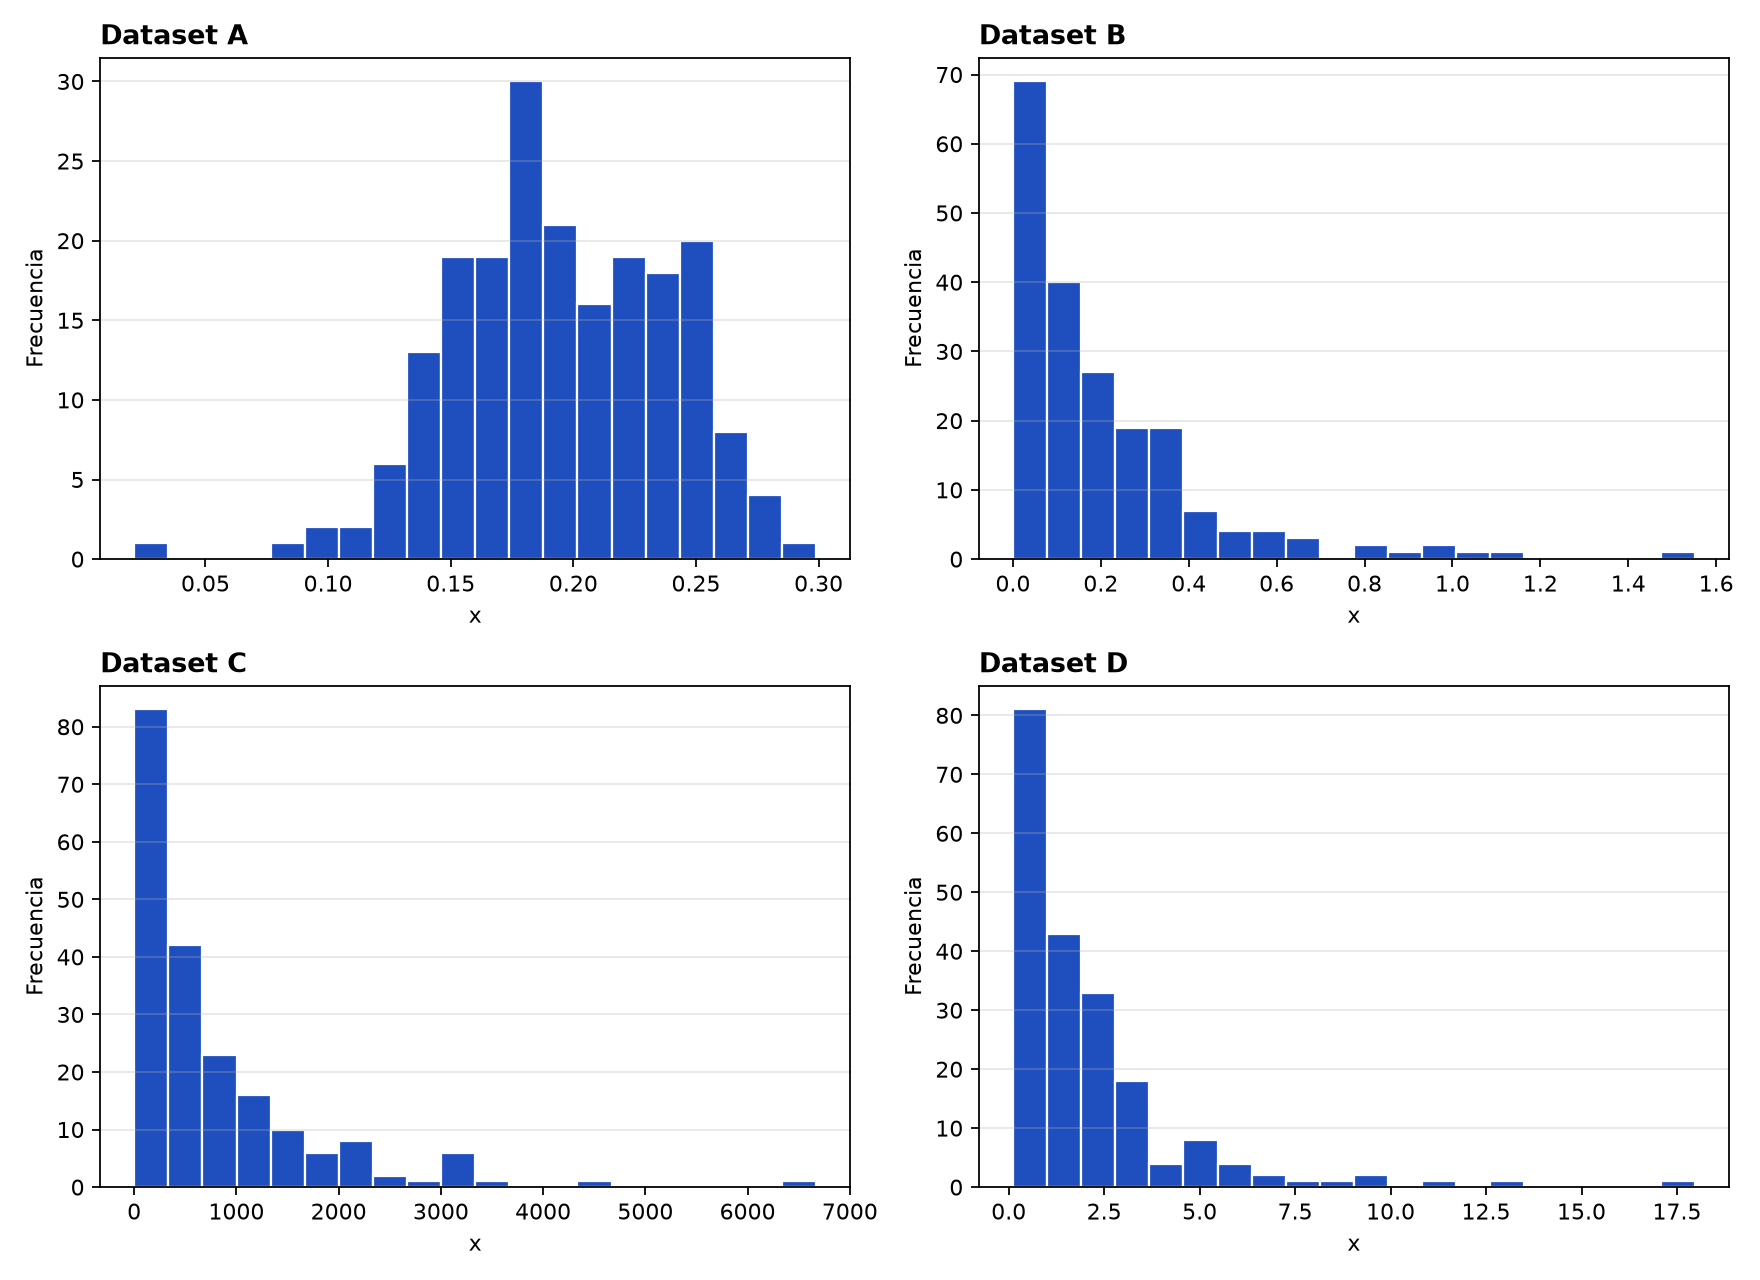
\includegraphics[width=0.82\textwidth]{histogramas.png}
\caption{Histogramas de los conjuntos A, B, C y D con 20 particiones.}
\label{fig:hist}
\end{figure*}

La Tabla~\ref{tab:desc} reúne las medidas que pide la guía. Se añaden el coeficiente de variación (CV), la asimetría y el exceso de curtosis, que ayudan a elegir las familias candidatas. Varianza y desviación estándar son muestrales (denominador $n-1$). La Fig.~\ref{fig:hist} muestra los histogramas.

\textbf{A} es casi simétrico (asimetría $-0.29$, media 0.195 y mediana 0.192) y poco disperso (CV de 0.22). Su histograma tiene forma de campana, con un solo valor aislado en 0.021. Ni la exponencial ni otra distribución con moda en cero lo describirán bien.

\textbf{B} tiene media 0.205 y desviación 0.229, de modo que su CV (1.12) está cerca de 1, el valor de la exponencial. La moda está en el primer intervalo, la mediana (0.138) queda muy por debajo de la media y la cola es larga hacia la derecha, con un máximo de 1.55. Todo esto es lo que se espera de tiempos entre llegadas de un proceso de Poisson con tasa cercana a 5.

\textbf{C} está en otra escala (media 762, máximo 6670). Tiene un CV de 1.21 y asimetría de 2.50. El histograma decrece desde cero, como una exponencial, pero con una cola larga.

\textbf{D} es el más asimétrico (3.18) y el de colas más pesadas (curtosis 14.5). Su moda no está en cero sino entre 0.5 y 1, lo que apunta a una lognormal o una log-logística más que a una exponencial.

Estas medidas no dicen nada sobre el orden de los datos. Las cifras de A serían las mismas si se barajara la muestra, y las de C no revelan que su media cambia con el tiempo. Eso se examina en el punto 5.2.

%--------------------------------------------------------------------
\section{Análisis de datos de entrada (punto 5.2)}
Las Figs.~\ref{fig:sec} a~\ref{fig:mm} muestran, para los cuatro conjuntos, la secuencia de valores y las cinco gráficas que pide la guía. La Tabla~\ref{tab:iid} resume las correlaciones y las medias por mitades.

\begin{figure}[t]
\centering
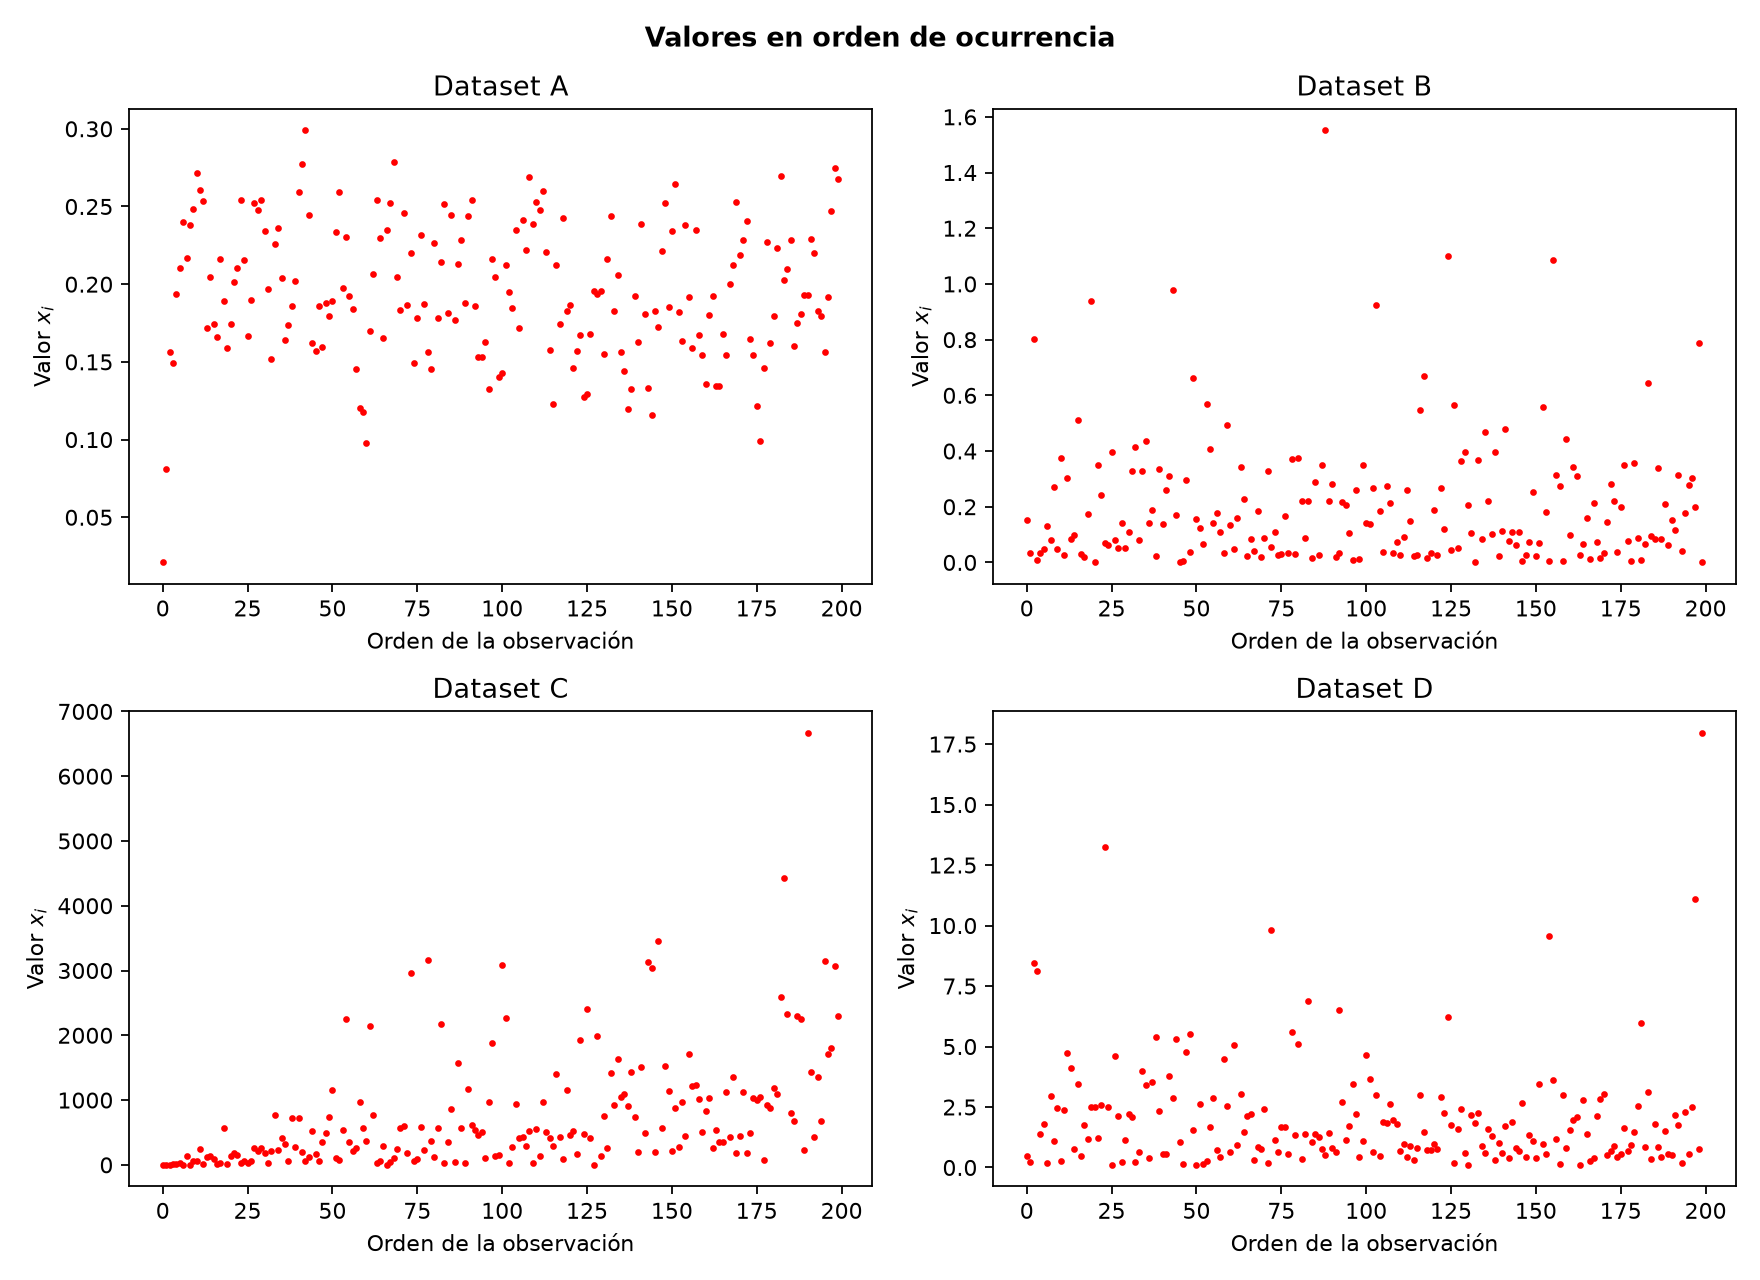
\includegraphics[width=\columnwidth]{secuencia.png}
\caption{Valores en orden de ocurrencia.}
\label{fig:sec}
\end{figure}

\begin{figure}[t]
\centering
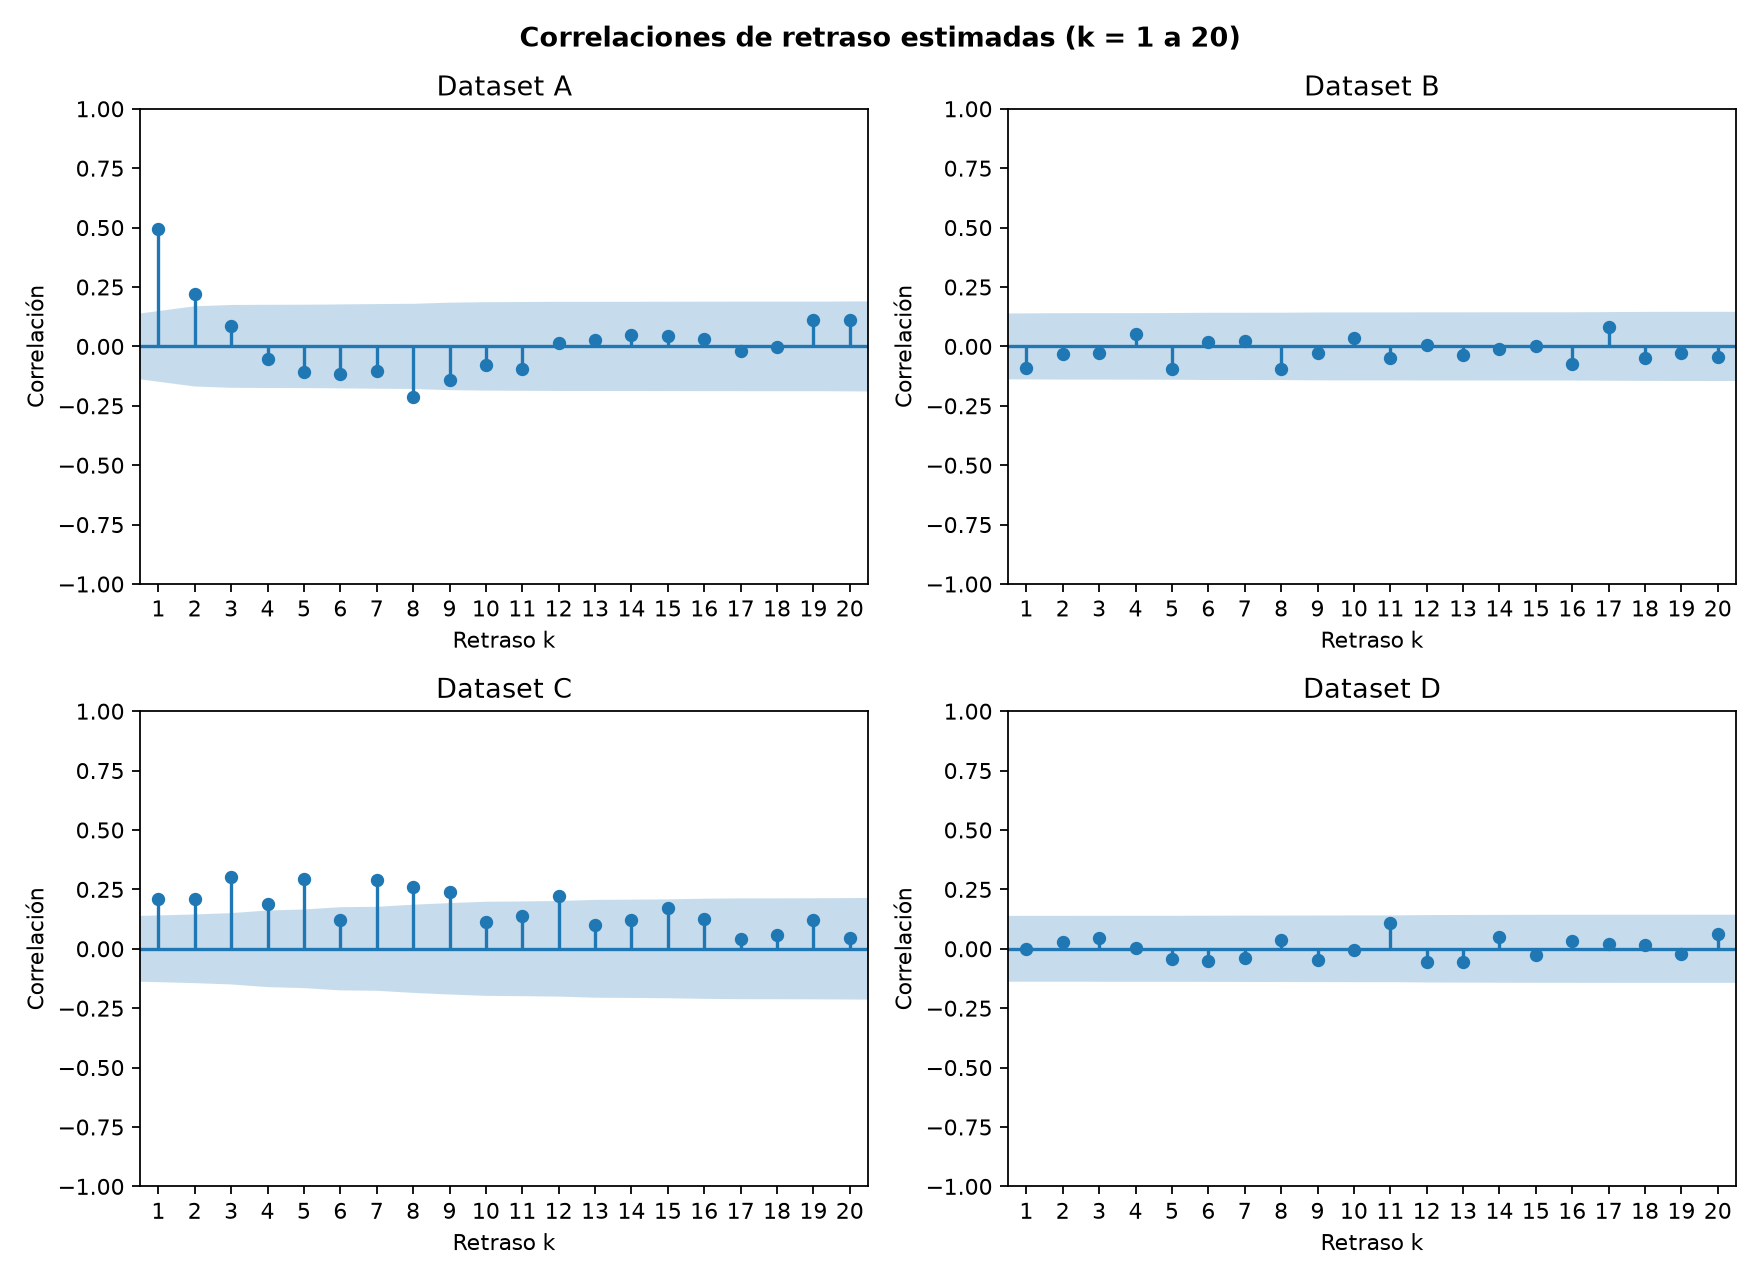
\includegraphics[width=\columnwidth]{correlaciones.png}
\caption{(a) Correlaciones de retraso estimadas, $k=1$ a 20. La franja sombreada es la banda de confianza del 95\,\% de \texttt{statsmodels}.}
\label{fig:acf}
\end{figure}

\begin{figure}[t]
\centering
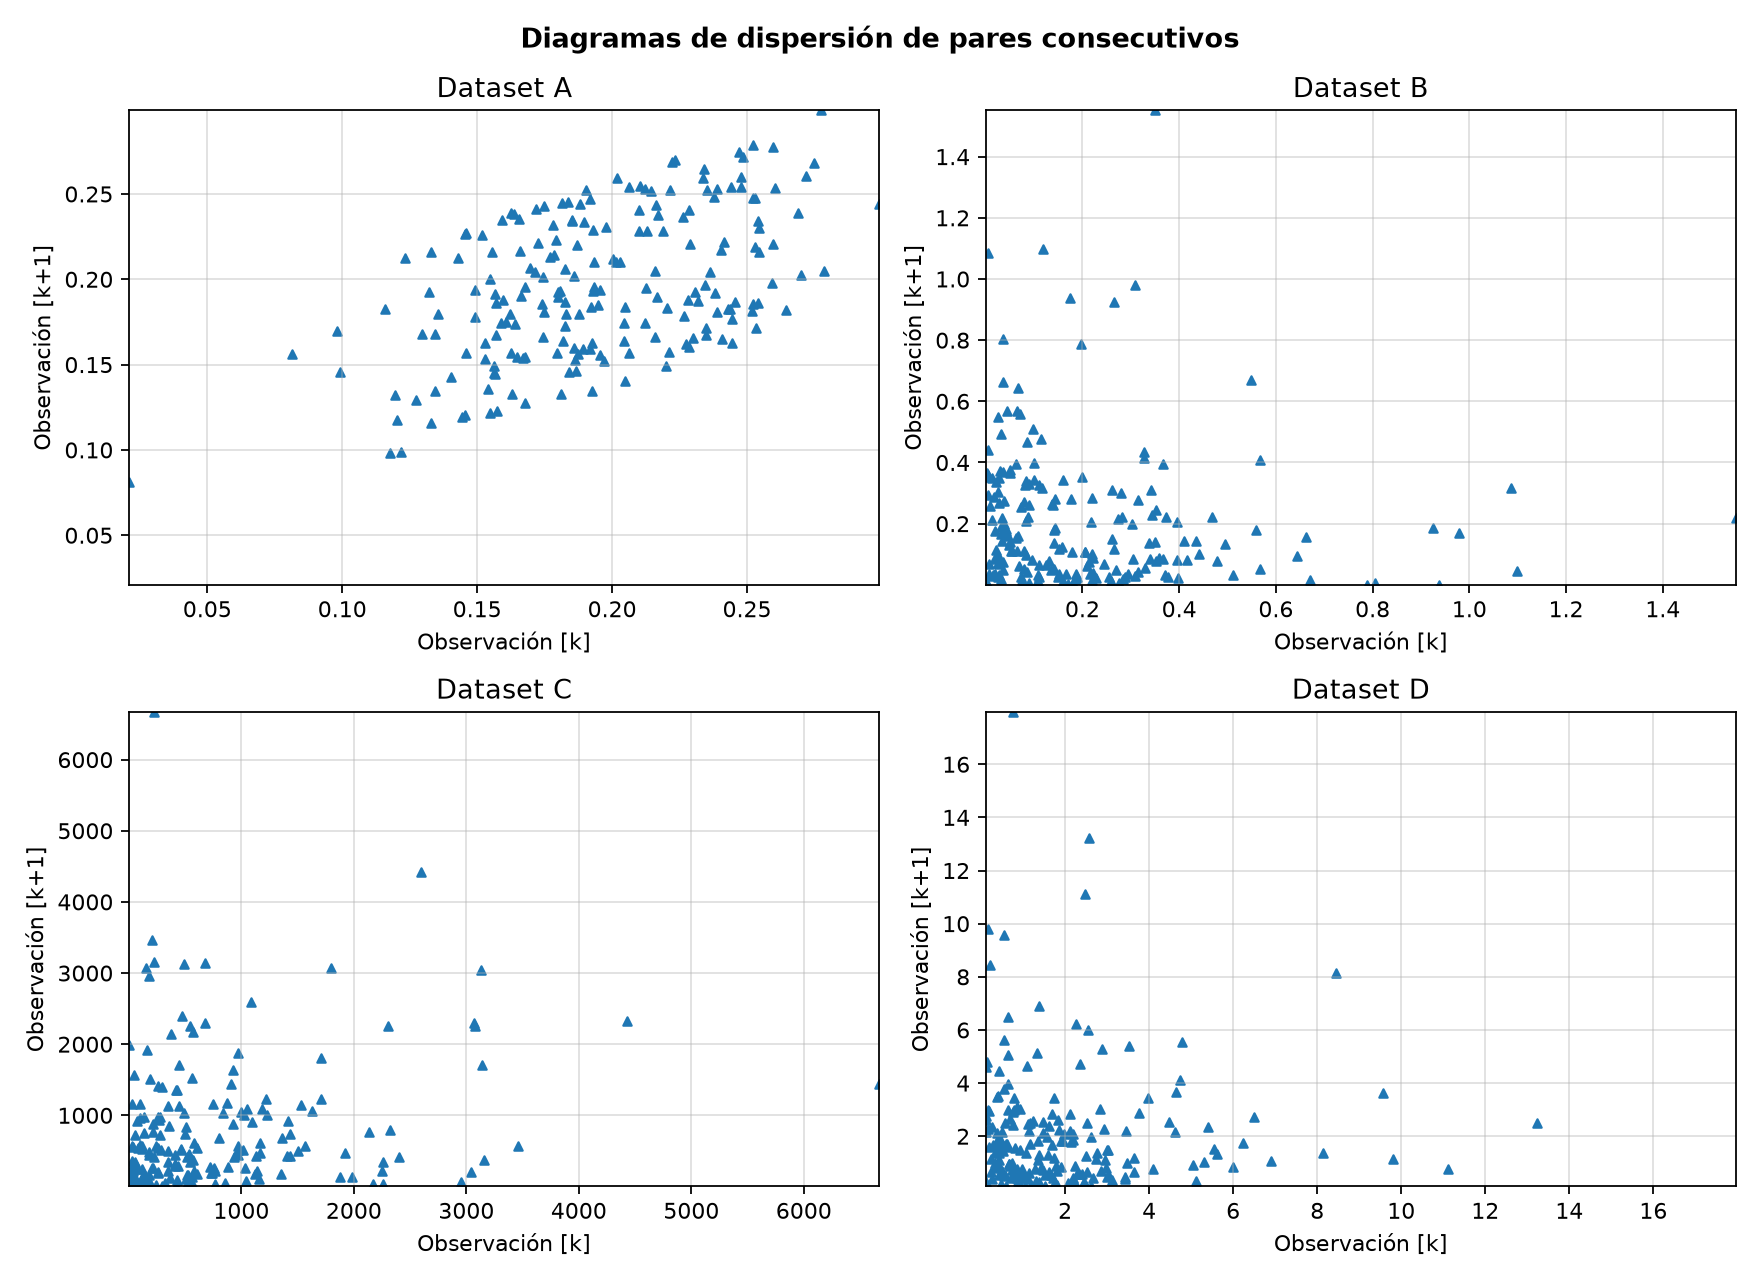
\includegraphics[width=\columnwidth]{dispersion.png}
\caption{(b) Diagramas de dispersión de pares consecutivos $(x_k,x_{k+1})$.}
\label{fig:disp}
\end{figure}

\begin{figure}[t]
\centering
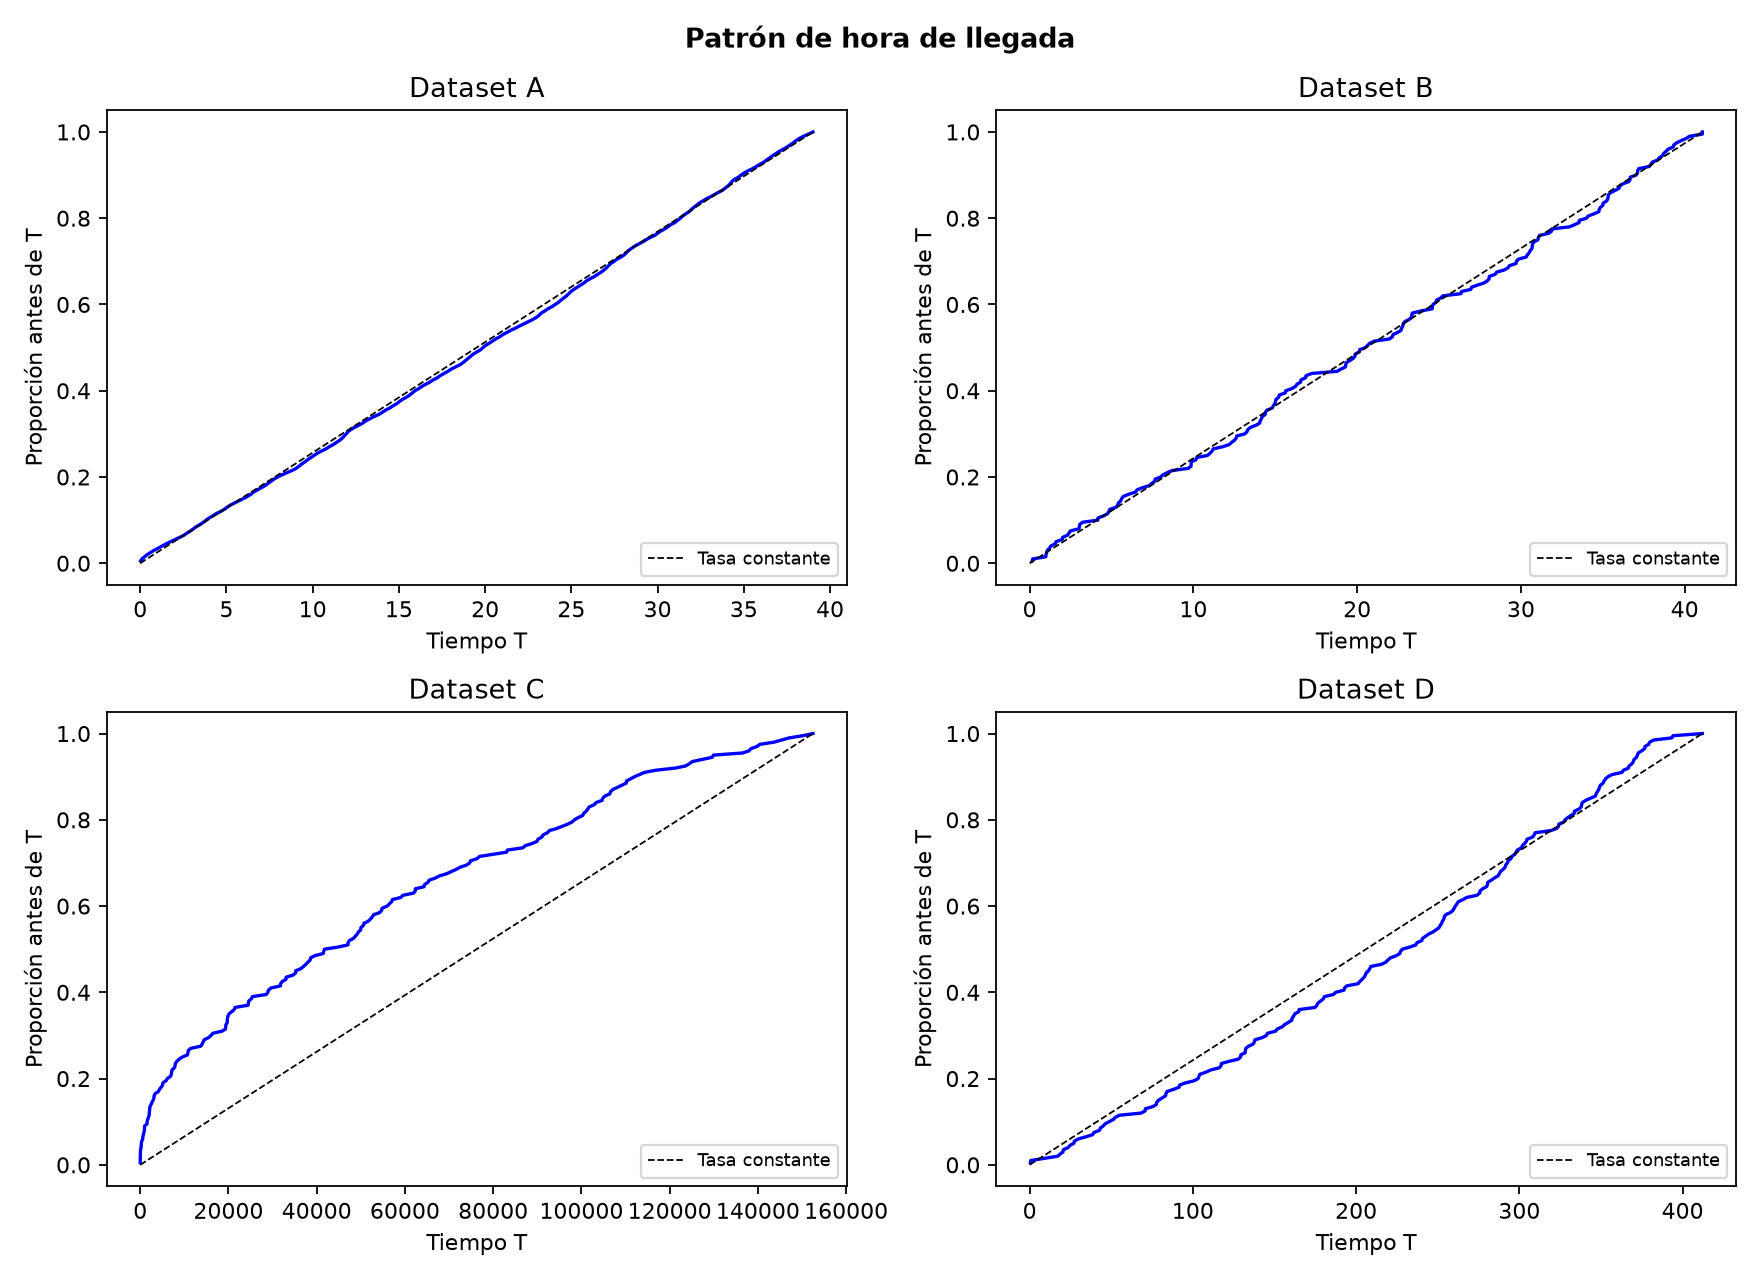
\includegraphics[width=\columnwidth]{patron_llegadas.png}
\caption{(c) Patrón de hora de llegada: proporción de llegadas antes de $T$. La línea punteada corresponde a una tasa constante.}
\label{fig:patron}
\end{figure}

\begin{figure}[t]
\centering
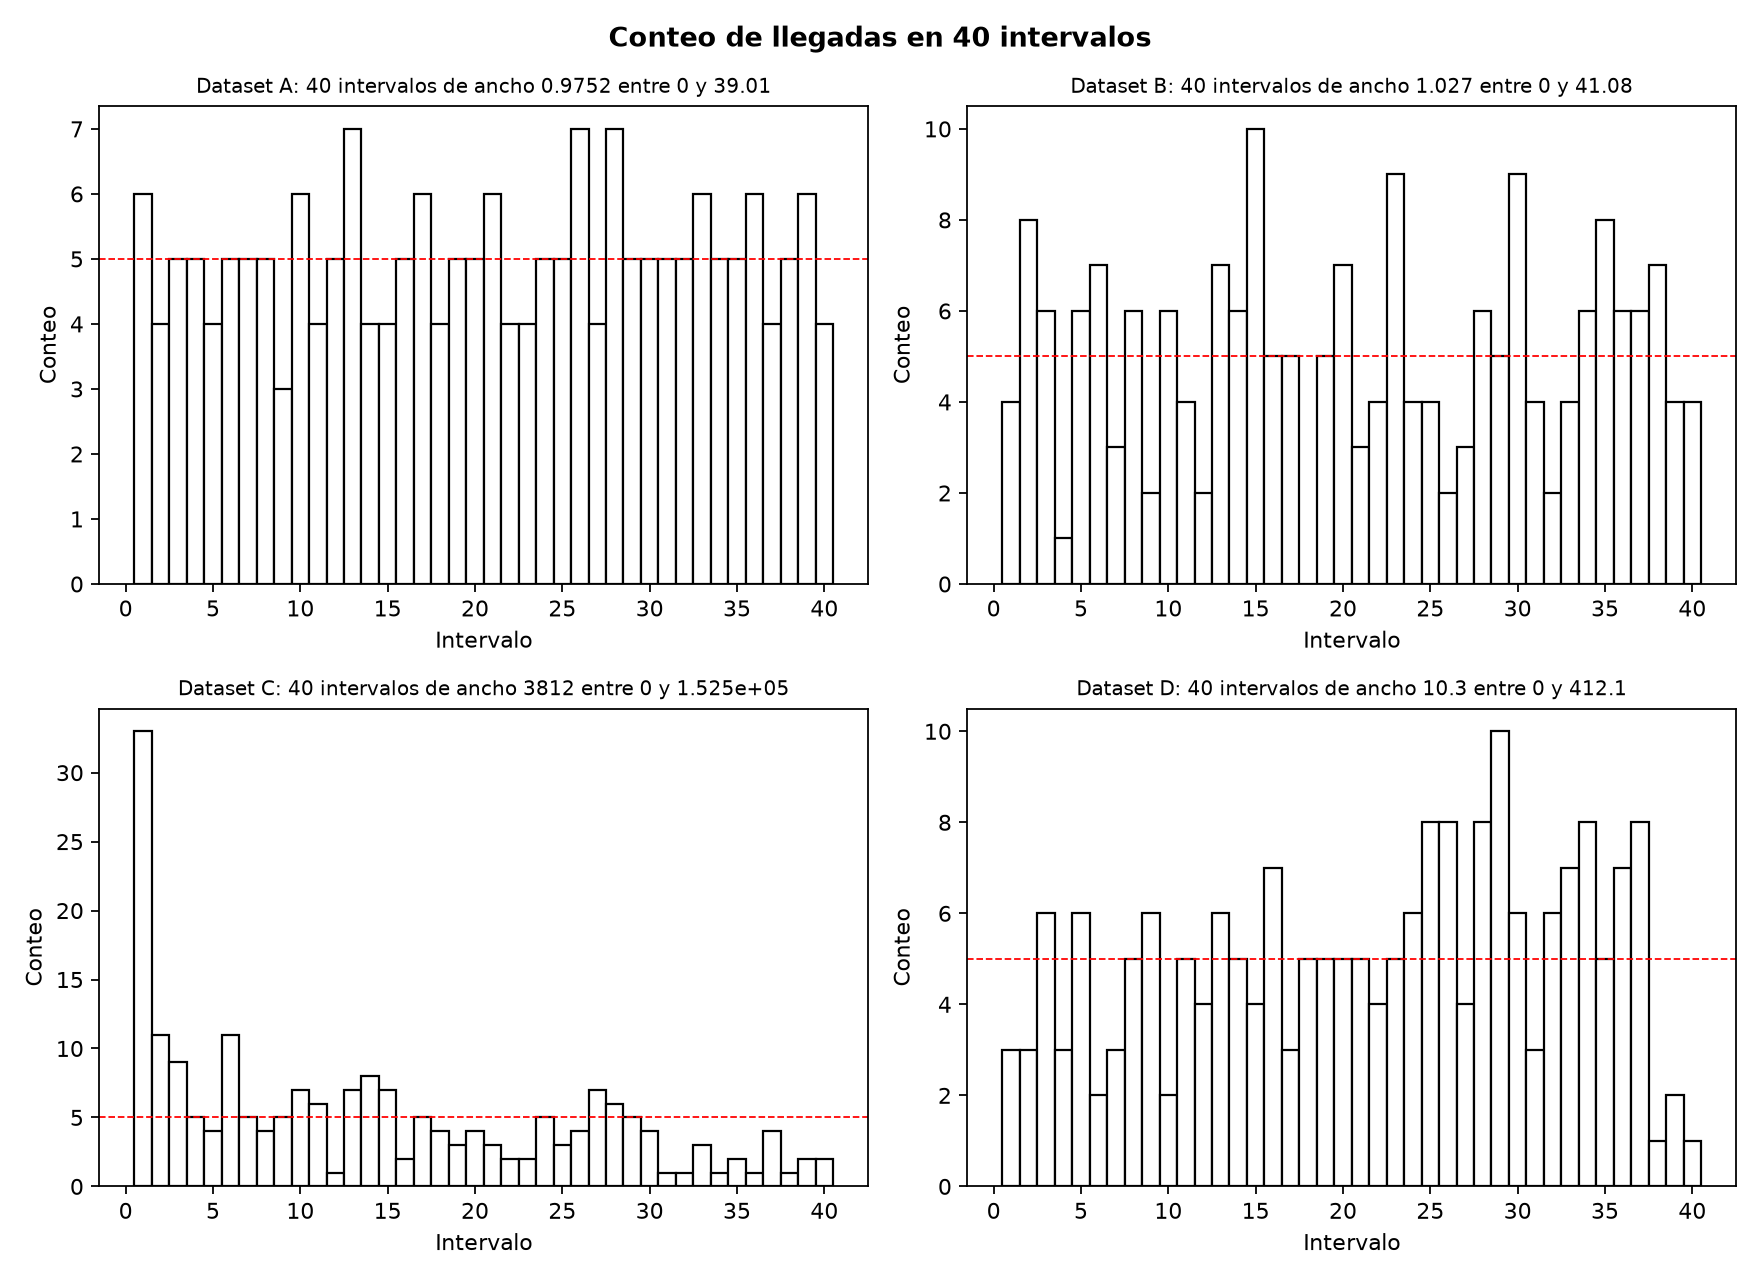
\includegraphics[width=\columnwidth]{conteos.png}
\caption{(d) Conteo de llegadas en 40 intervalos de igual ancho. La línea roja es el conteo medio (5).}
\label{fig:conteos}
\end{figure}

\begin{figure}[t]
\centering
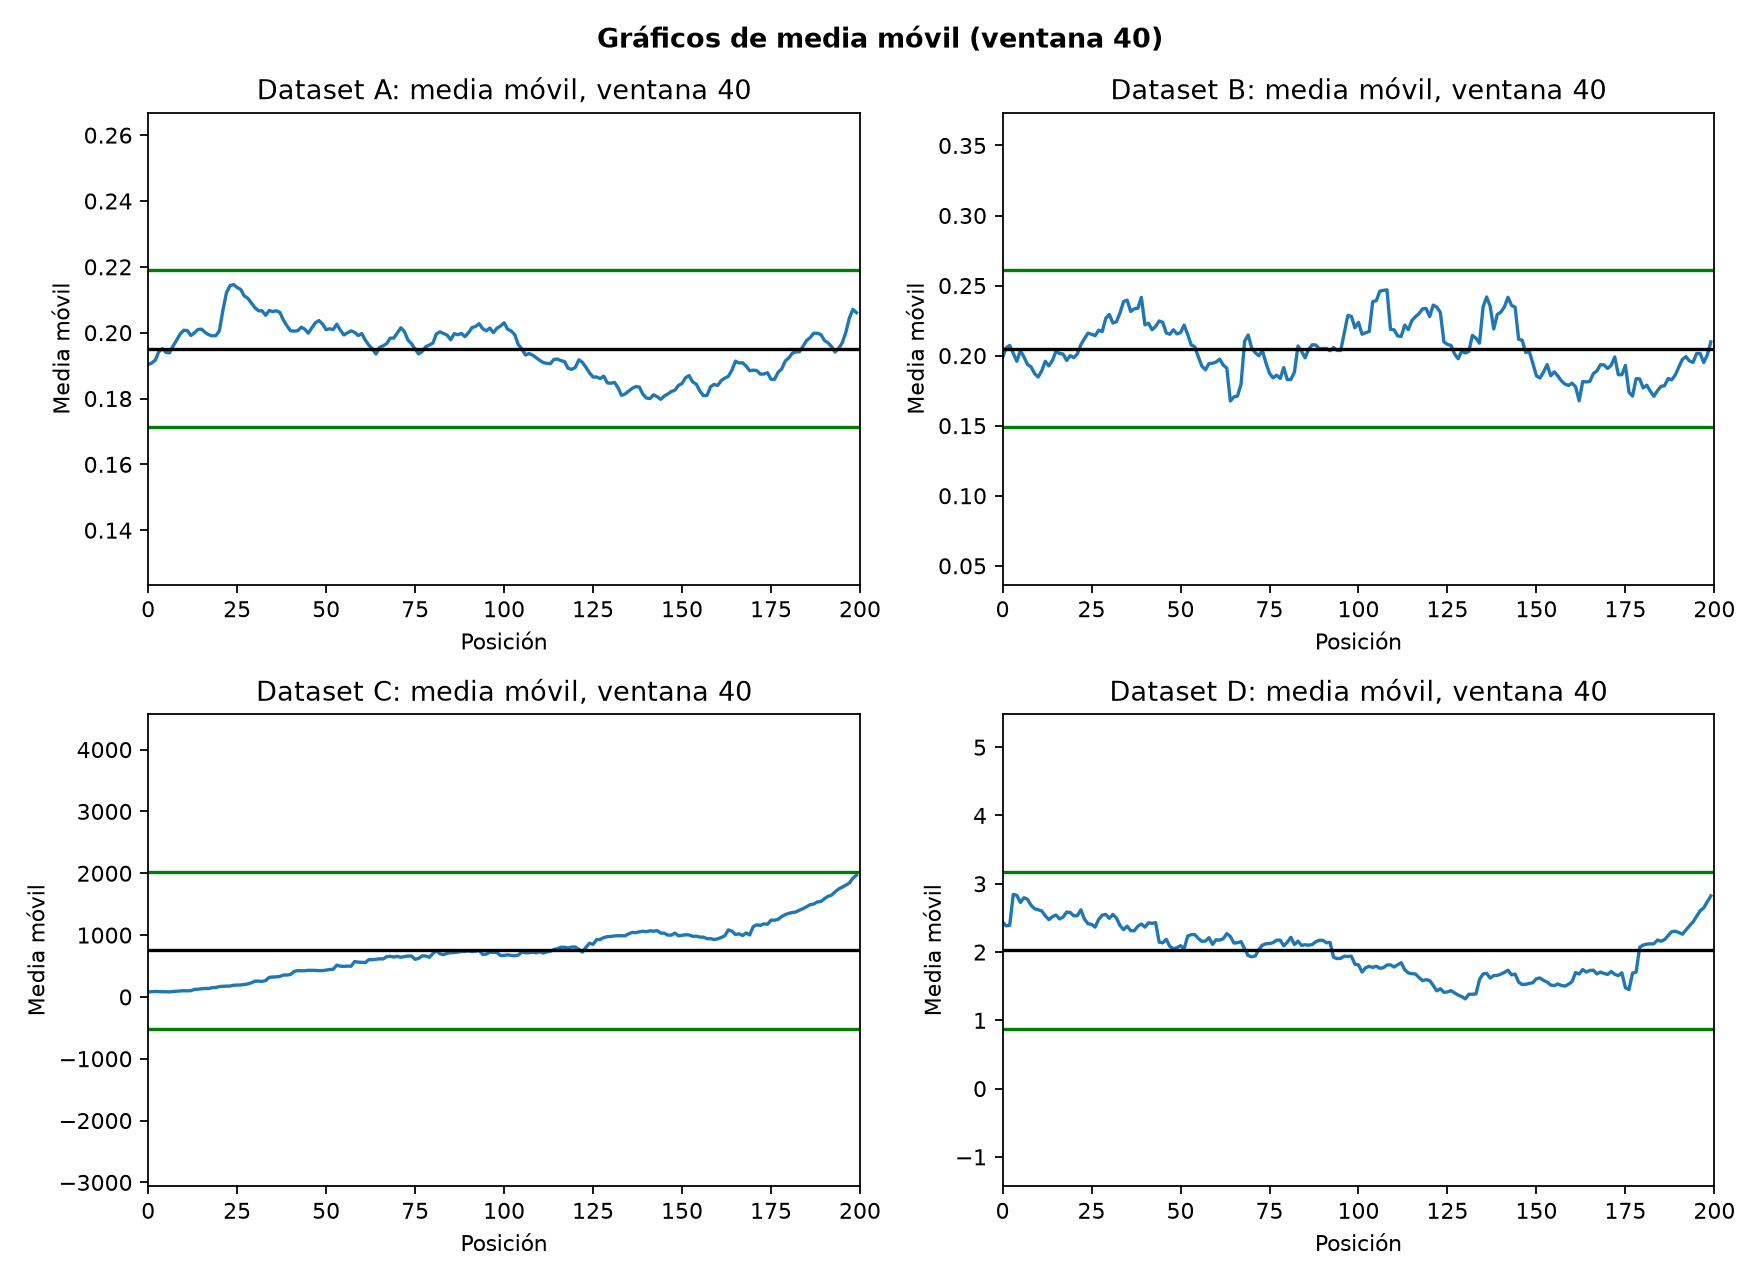
\includegraphics[width=\columnwidth]{media_movil.png}
\caption{(e) Media móvil con ventana de 40 datos. Línea negra: media de la curva; verdes: $\pm3$ desviaciones estándar de la curva.}
\label{fig:mm}
\end{figure}

\begin{table}[t]
\caption{Autocorrelaciones y medias por mitades}
\label{tab:iid}
\centering\footnotesize
\setlength{\tabcolsep}{3pt}
\begin{tabular}{@{}lrrrr@{}}
\toprule
Medida & A & B & C & D \\
\midrule
\tabla{independencia}
\bottomrule
\end{tabular}
\end{table}

\subsection{Dataset A: estacionario pero correlacionado}
Es el único con correlación positiva clara en los primeros retrasos: $r_1=0.49$ y $r_2=0.22$, muy por fuera de la banda (Fig.~\ref{fig:acf}). En el diagrama de dispersión (Fig.~\ref{fig:disp}) los puntos se alinean a lo largo de la diagonal que sube de izquierda a derecha, que es la señal de correlación positiva descrita en clase, y en la secuencia (Fig.~\ref{fig:sec}) se ven rachas de valores altos y bajos. En cambio, la distribución es estable. El patrón de llegadas es prácticamente la recta de tasa constante, los conteos por intervalo varían poco alrededor de 5 y la media móvil se queda entre 0.18 y 0.21, dentro de su banda. Las dos mitades tienen medias de 0.199 y 0.191. A se parece al conjunto 6 del cuaderno de clase, en el que cada valor es un promedio ponderado del anterior y un uniforme. \emph{Conclusión:} no es IID, porque falla la independencia.

\subsection{Dataset B: compatible con IID}
Todas sus correlaciones están dentro de la banda, con signos mezclados ($|r_k|\le0.094$). El diagrama de dispersión se concentra cerca del origen y se abre hacia los ejes, sin alinearse en ninguna diagonal, como en el ejemplo exponencial de clase. El patrón de llegadas sigue la recta, los conteos fluctúan entre 1 y 10 sin tendencia y la media móvil oscila sin salir de la banda. Las mitades tienen medias de 0.205 y 0.206. \emph{Conclusión:} no hay evidencia contra el supuesto IID.

\subsection{Dataset C: no estacionario}
El patrón de llegadas es la gráfica más clara: la curva es cóncava y queda muy por encima de la recta, de modo que el 34\,\% de las llegadas ocurre en el primer 13\,\% del horizonte. Los conteos lo confirman: 33 llegadas en el primer intervalo y entre 1 y 4 en los últimos diez. La tasa de llegada cae con el tiempo, es decir, los tiempos entre llegadas crecen. La media móvil sube casi de forma continua, de unos 100 a unos 2000, y las medias por cuartos son 191, 644, 964 y 1251. Las correlaciones son positivas en 8 de los primeros 10 retrasos y decaen lentamente. Esto no indica que un valor dependa del anterior, sino que la media sube: cuando la media tiene tendencia, valores cercanos tienden a ser parecidos. \emph{Conclusión:} no es IID; falla la estabilidad de la distribución.

\subsection{Dataset D: compatible con IID}
Sus correlaciones son las más pequeñas de los cuatro ($|r_k|\le0.053$ en los retrasos 1 a 10) y la dispersión no muestra patrón. La media de la segunda mitad (1.84) es algo menor que la de la primera (2.28), y el patrón de llegadas se separa de la recta hasta 0.07. Con un CV de 1.13, el error estándar de la media de 50 datos es de unos 0.33, así que las medias por cuartos (2.59, 1.98, 1.52 y 2.16) caben en esa variación sin una tendencia definida. La media móvil también se queda dentro de su banda. Hay que tener cuidado al leerla: su subida final se debe a dos valores grandes entre los cuatro últimos (11.11 y 17.97), y en ese extremo la ventana promedia menos datos. \emph{Conclusión:} no hay evidencia clara contra el supuesto IID; la variación de la media es moderada y compatible con el azar.

%--------------------------------------------------------------------
\section{Ajuste de curvas (punto 5.3)}
Las Tablas~\ref{tab:ajA} a~\ref{tab:ajD} muestran los nueve ajustes de cada conjunto, con las tres mejores por AIC en negrita. La Fig.~\ref{fig:top3} superpone esas tres al histograma y la Fig.~\ref{fig:qq} compara los cuantiles de la mejor con los observados. En las tablas, $\beta$ es el parámetro de escala, $\alpha$ el de forma de la gamma, $c$ el de forma de la Weibull y la log-logística, y $\xi$ el de forma de la Pareto generalizada. En la lognormal, $\sigma$ es la desviación del logaritmo y $\beta=e^{\mu}$. En la gaussiana inversa se usa la parametrización de SciPy, con media $\mu\beta$.

\begin{table*}[t]
\caption{Bondad de ajuste para el conjunto de datos A}
\label{tab:ajA}
\centering\footnotesize
\begin{tabular}{@{}llrrrr@{}}
\toprule
Distribución & Parámetros & SSE & AIC & BIC & KS $D$ \\
\midrule
\tabla{ajuste_A}
\bottomrule
\end{tabular}

\vspace{8pt}
\caption{Bondad de ajuste para el conjunto de datos B}
\label{tab:ajB}
\begin{tabular}{@{}llrrrr@{}}
\toprule
Distribución & Parámetros & SSE & AIC & BIC & KS $D$ \\
\midrule
\tabla{ajuste_B}
\bottomrule
\end{tabular}
\end{table*}

\begin{table*}[t]
\caption{Bondad de ajuste para el conjunto de datos C}
\label{tab:ajC}
\centering\footnotesize
\begin{tabular}{@{}llrrrr@{}}
\toprule
Distribución & Parámetros & SSE & AIC & BIC & KS $D$ \\
\midrule
\tabla{ajuste_C}
\bottomrule
\end{tabular}

\vspace{8pt}
\caption{Bondad de ajuste para el conjunto de datos D}
\label{tab:ajD}
\begin{tabular}{@{}llrrrr@{}}
\toprule
Distribución & Parámetros & SSE & AIC & BIC & KS $D$ \\
\midrule
\tabla{ajuste_D}
\bottomrule
\end{tabular}
\end{table*}

\begin{figure*}[t]
\centering
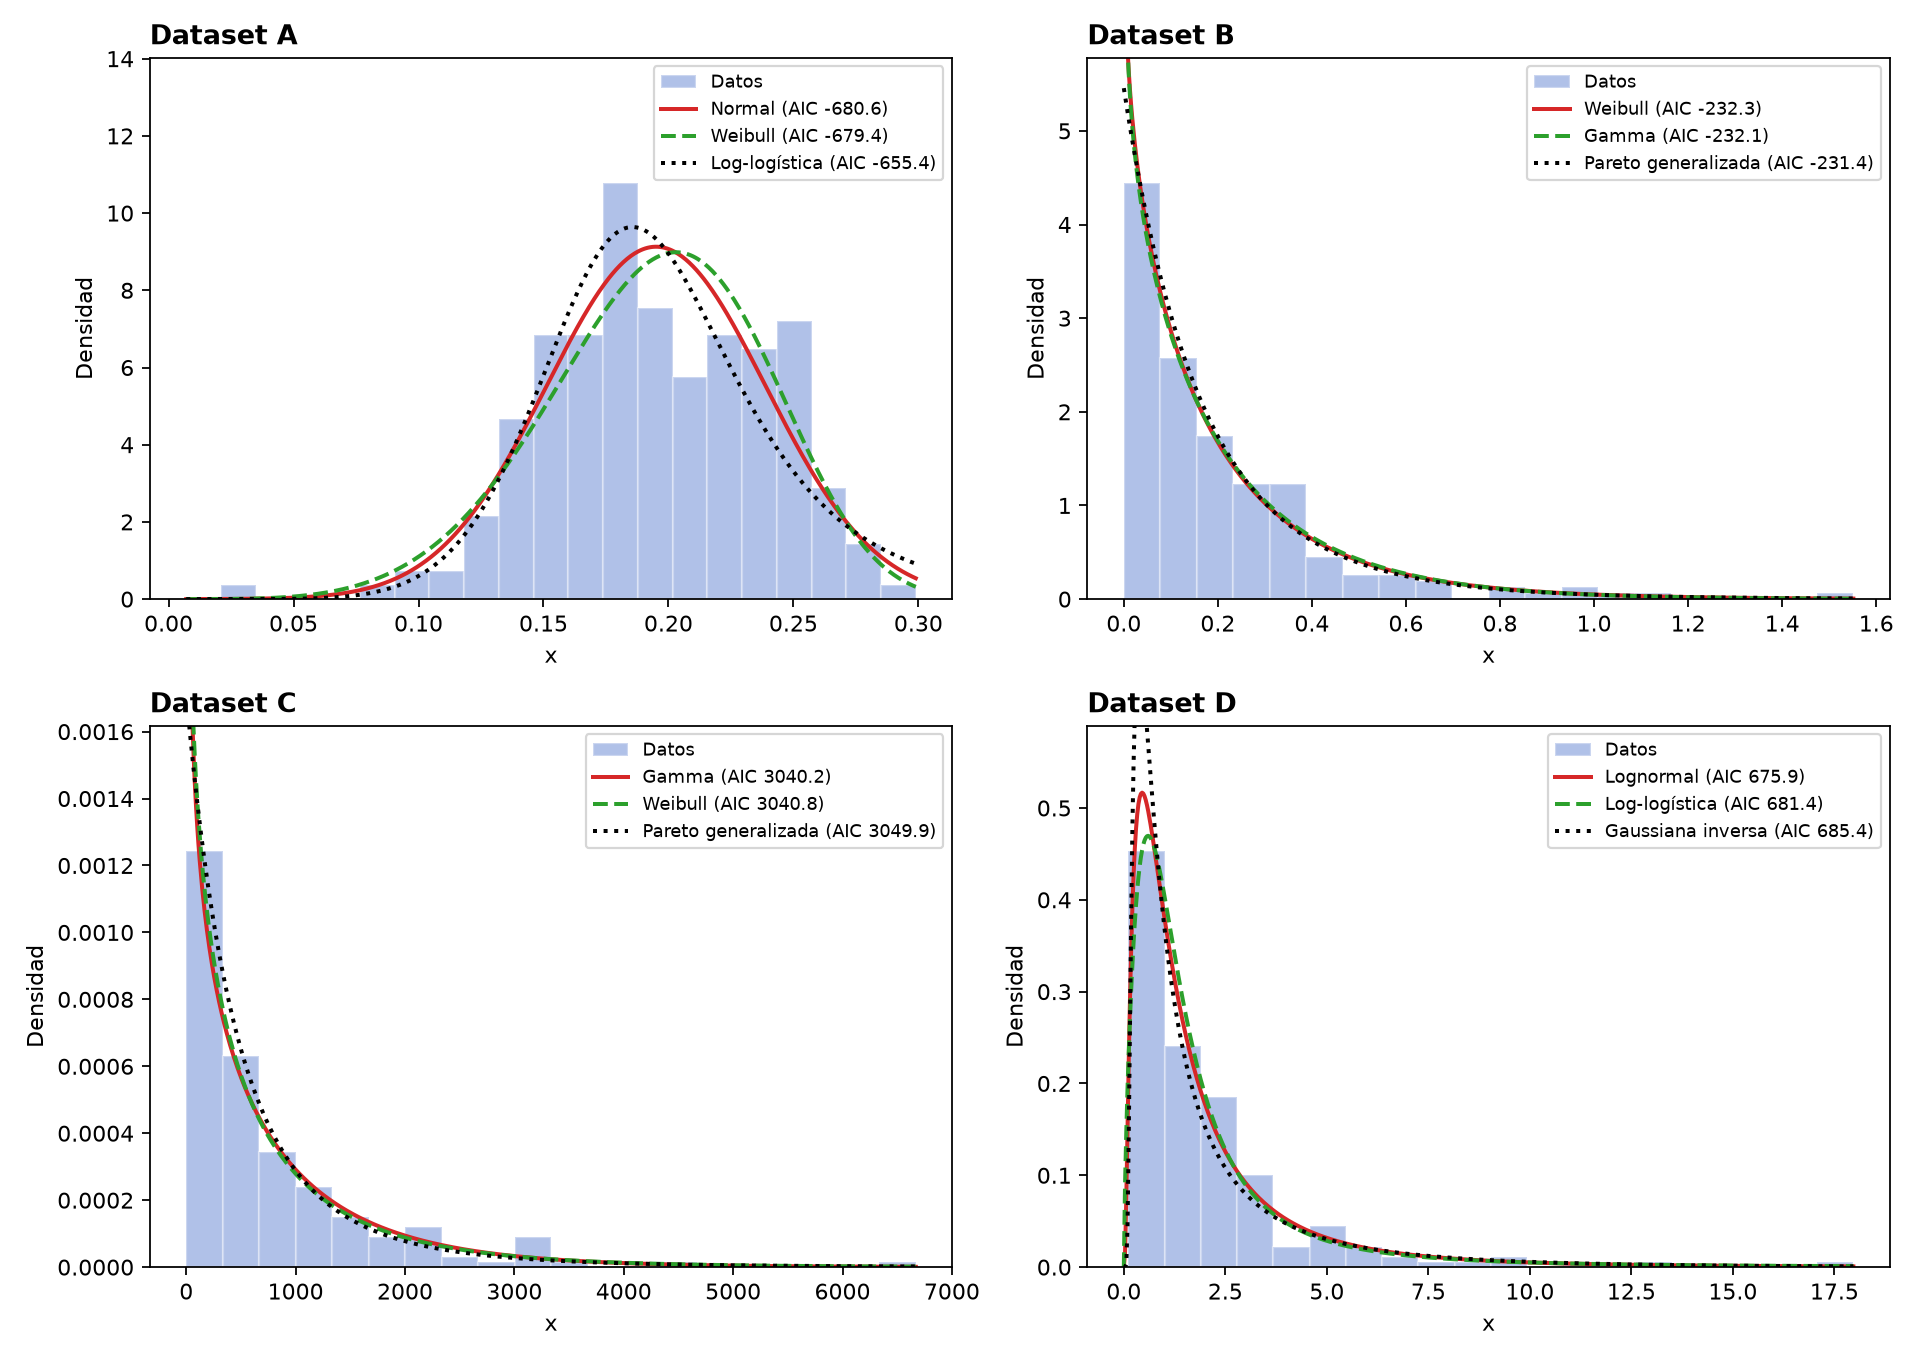
\includegraphics[width=0.72\textwidth]{top3_todos.png}
\caption{Histograma de cada conjunto (densidad, 20 particiones) con las tres distribuciones de menor AIC. En B y C el eje vertical se recortó porque las densidades con forma menor que 1 tienden a infinito en cero.}
\label{fig:top3}
\end{figure*}

\begin{figure*}[t]
\centering
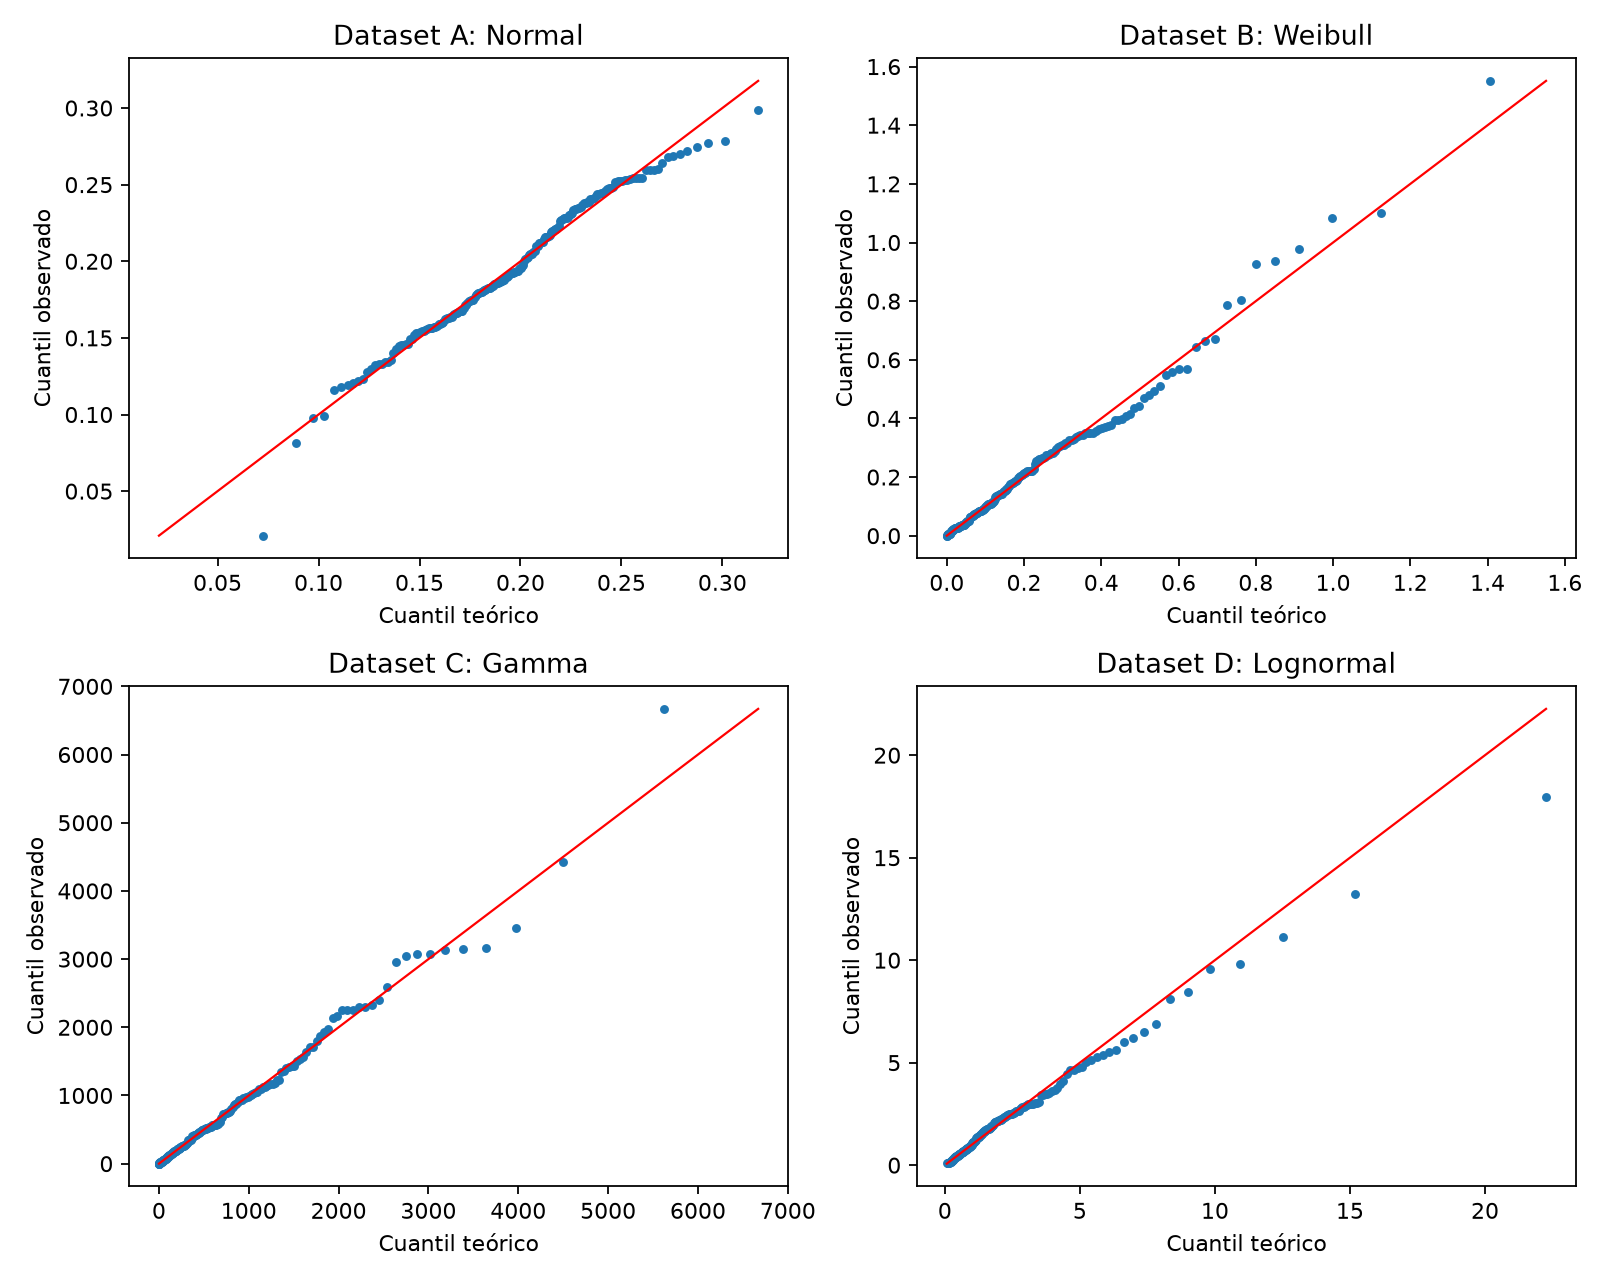
\includegraphics[width=0.6\textwidth]{qq_mejor.png}
\caption{Gráficas Q-Q de la distribución de menor AIC en cada conjunto.}
\label{fig:qq}
\end{figure*}

\subsection{Dataset A}
Las tres mejores son la normal ($\mu=0.195$, $\sigma=0.0437$; AIC $-680.59$), la Weibull ($c=5.07$, $\beta=0.212$; AIC $-679.36$) y la log-logística ($c=7.29$, $\beta=0.193$; AIC $-655.44$). La normal y la Weibull empatan en la práctica ($\Delta\mathrm{AIC}=1.2$), pero la normal también tiene menor SSE y menor $D$. Las distribuciones con moda en cero quedan descartadas: la exponencial tiene un AIC de $-251.8$ y $D=0.43$. Aunque la normal admite valores negativos, la probabilidad de uno es $\Phi(-0.195/0.0437)\approx4\times10^{-6}$, despreciable en la práctica. La gráfica Q-Q muestra que la cola superior de los datos es algo más corta que la de la normal (el máximo es 0.299) y que el valor 0.021 queda aislado abajo.

\emph{Selección:} normal $\mathcal{N}(0.195,\,0.0437^2)$. Pero la normal solo describe la distribución marginal. Si se generan valores independientes de ella, la simulación pierde la correlación $r_1=0.49$ y producirá menos rachas de llegadas rápidas o lentas que el proceso real. Para respetar esa dependencia, una opción es un proceso autorregresivo de orden 1 con marginal normal, $X_k=\mu+\phi\,(X_{k-1}-\mu)+\varepsilon_k$ con $\phi\approx0.49$ y $\mathrm{Var}(\varepsilon_k)=\sigma^2(1-\phi^2)$, que conserva la media y la varianza estimadas.

\subsection{Dataset B}
Las tres mejores son la Weibull ($c=0.910$, $\beta=0.196$; AIC $-232.26$), la gamma ($\alpha=0.864$, $\beta=0.238$; AIC $-232.10$) y la Pareto generalizada ($\xi=0.108$, $\beta=0.183$; AIC $-231.39$). Las tres están a menos de 0.9 unidades de AIC entre sí, y la exponencial, cuarta, queda a 1.1 de la primera. Las tres tienen un parámetro de forma cercano al caso exponencial (forma 1 en Weibull y gamma, $\xi=0$ en la Pareto generalizada), así que en realidad describen casi la misma curva, como se ve en la Fig.~\ref{fig:top3}. Por BIC, que castiga el parámetro adicional, la exponencial ($\beta=0.2054$) es la mejor ($-227.83$ frente a $-225.67$ de la Weibull).

\emph{Selección:} entre las tres, la Weibull con $c=0.91$ y $\beta=0.196$, que tiene el menor AIC, el menor SSE (0.276) y el menor $D$ (0.035), con una gráfica Q-Q casi sobre la diagonal. Como su forma está tan cerca de 1, una exponencial con media 0.205 (llegadas de Poisson con tasa de unos 4.9) es una simplificación razonable, y es la que prefiere el BIC. El conjunto se parece al conjunto 1 del cuaderno de clase (exponencial con media 0.2).

\subsection{Dataset C}
Las tres mejores son la gamma ($\alpha=0.706$, $\beta=1080$; AIC 3040.22), la Weibull ($c=0.801$, $\beta=676$; AIC 3040.81) y la Pareto generalizada ($\xi=0.245$, $\beta=583.7$; AIC 3049.87). Gamma y Weibull empatan; la Weibull tiene menor $D$ y la Pareto generalizada, el menor SSE. Que las formas sean menores que 1 indica más dispersión que una exponencial, y eso es justamente lo que produce mezclar tiempos cortos del comienzo con tiempos largos del final.

Para comprobarlo, el cuaderno repite el ajuste en cada mitad. En la primera (media 418), la mejor es una Weibull con $c=0.72$ y $\beta=335$. En la segunda (media 1107), la gamma ($\alpha=1.21$) y la exponencial ($\beta=1107$) empatan, con $\Delta\mathrm{AIC}=0.07$, y por BIC gana la exponencial. Los parámetros cambian mucho entre las mitades, lo que confirma la falta de estacionariedad.

\emph{Selección:} de las tres, la gamma ($\alpha=0.706$, $\beta=1080$), por ser la de menor AIC y BIC. Como modelo único para la simulación no se recomienda: generaría tiempos con la dispersión correcta pero en un orden aleatorio, sin la tendencia creciente. Lo adecuado es un modelo no estacionario: un proceso de Poisson no homogéneo con una tasa decreciente estimada a partir de los conteos de la Fig.~\ref{fig:conteos}, o distribuciones distintas por períodos (la segunda mitad es casi exponencial). Si el estudio solo cubre un período, se ajusta la distribución con los datos de ese período, como recomienda el material de clase.

\subsection{Dataset D}
Las tres mejores son la lognormal ($\sigma=1.019$, $\beta=1.273$, es decir $\mu=\ln1.273=0.241$; AIC 675.89), la log-logística ($c=1.705$, $\beta=1.31$; AIC 681.40) y la gaussiana inversa (AIC 685.40). Aquí la ventaja de la lognormal es clara: 5.5 unidades de AIC y 5.5 de BIC sobre la segunda. La log-logística tiene un SSE algo menor (0.0060 frente a 0.0069) y un $D$ ligeramente menor, pero son diferencias pequeñas frente a la de verosimilitud. En la Q-Q, la lognormal sigue la diagonal hasta $x\approx8$; los valores más altos quedan algo por debajo, de modo que el modelo predice una cola algo más pesada que la observada. Con solo siete valores por encima de 8, esa zona es poco confiable. La exponencial y la gamma tienen la moda en cero o casi en cero y no reproducen el pico entre 0.5 y 1.

\emph{Selección:} lognormal con $\mu=0.241$ y $\sigma=1.019$ (en SciPy, \texttt{lognorm(s=1.019, scale=1.273)}). El conjunto se parece al conjunto 3 del cuaderno de clase (lognormal con parámetro de forma 1.0).

\subsection{Consistencia entre medidas}
AIC y BIC dieron el mismo orden en A, C y D, y en B solo cambiaron el lugar de la exponencial. El SSE coincidió con AIC en el primer lugar únicamente en B; es sensible a las particiones y pesa poco las colas, donde está la diferencia entre modelos. Por eso, como recomienda el material de clase, la elección no se basó en una sola medida, sino en las tres junto con $D$, las gráficas y el rango de los datos.

%--------------------------------------------------------------------
\section{Conclusiones}
El paso más importante fue comprobar el supuesto IID antes de ajustar. Con solo la Tabla~\ref{tab:desc} y los histogramas, A y C parecían candidatos normales para un ajuste. Las gráficas de 5.2 mostraron que A está correlacionado ($r_1=0.49$) y que C no es estacionario (su media se multiplica por 2.65 entre mitades). En ambos casos la distribución con mejor AIC describe la marginal, pero no el proceso.

Para los conjuntos IID, el ajuste dio modelos claros: B es esencialmente exponencial (Weibull con forma 0.91, o exponencial de media 0.205 si se prefiere un solo parámetro) y D es lognormal ($\mu=0.241$, $\sigma=1.019$). En B, la Weibull, la gamma y la Pareto generalizada quedaron separadas por menos de una unidad de AIC. En casos así hay que preferir el modelo más simple que tenga sentido con el origen de los datos.

Las medidas de ajuste no siempre coinciden, y el SSE depende de cómo se construya el histograma. Usar varias medidas, las gráficas Q-Q y el rango físico de la variable da una elección más sólida que cualquier medida por separado.

%--------------------------------------------------------------------
\balance
\begin{thebibliography}{1}
\bibitem{guia} A. A. Cruz Roa, ``FO-DOC-112. Práctica 04: Análisis de datos de entrada y ajuste de datos a distribuciones de probabilidad,'' Universidad de los Llanos, 5 de abril de 2024.
\bibitem{banks98} J. Banks, Ed., \emph{Handbook of Simulation: Principles, Methodology, Advances, Applications, and Practice}. New York: John Wiley \& Sons, 1998, cap. 3.
\bibitem{clase} A. A. Cruz Roa, ``3. Input Data Analysis,'' presentación de clase, Simulación Computacional, Universidad de los Llanos.
\bibitem{amat2021} J. Amat Rodrigo, ``Ajuste y selección de distribuciones con Python,'' 2021. [En línea]. Disponible: \url{https://www.cienciadedatos.net/documentos/pystats01-ajuste-distribuciones-python.html}. doi: 10.5281/zenodo.10006330.
\bibitem{scipy} P. Virtanen \emph{et al.}, ``SciPy 1.0: Fundamental algorithms for scientific computing in Python,'' \emph{Nature Methods}, vol. 17, pp. 261--272, 2020.
\end{thebibliography}

\end{document}
